\chapter{Alternativen}
\label{ch:alt}
Folgendes Kapitel soll die Vor- und Nachteile von möglichen Alternativen zur Datenkommunikation via Bluetooth aufzeigen.

\section{Kabel}
Die einfachste und älteste Methode, um Daten auszutauschen, ist das Kabel.

\subsubsection{Vorteile}
%todo MAKE THIS SENTENCE
\hl1{Alleine durch das Trägermedium ist ein Kabel sicherer als z.B. Funk, da das Signal nur auf dem Kabel selbst erfolgt und nicht via Luft von überall zugegriffen werden kann.}
Zudem kann die Verbindung verschlüsselt werden, sodass bei langen und unüberschaubaren Verbindungen das Abhören massiv erschwert wird.
Kabel sind meistens sehr günstig, schnell, stromsparend und es können Standardstecker verwendet werden (z.B. \gls{usbLabel}).

\subsubsection{Nachteile}
Der grösste Nachteil eines Kabels liegt hauptsächlich im Bereich Mobilität.
Verwendete Kabel müssen transportiert und bei Gebrauch eingesteckt werden.
Oft erzwingen verschiedene Schnittstellen zudem den Einsatz zusätzlicher Hardware (weitere Kabel und Adapters), um den Gebrauchsanforderungen zu entsprechen.
Will man für wichtige Einsätze (z.B. Präsentationen) sicher gehen, dass alles reibungslos funktioniert, müssen oft mehrere Adapter bereitgestellt werden.
Dieser Bedarf an Hardware wirkt sich natürlich auch finanziell aus.
Zudem sind  die jeweiligen Geräte direkt mit dem Kommunikationspartner verbunden.
Dies ist beispielsweise bei der Nutzung eines Smartphone kaum vorstellbar.

Diese genannten Nachteile des Kabels galten als Motivationsursprung für die Entwicklung drahtloser Kommunikation.

\section{Drahtlose Kommunikation}

Als \textit{drahtlose Kommunikation} wird der Teil einer Verbindung bezeichnet, der oft über elektromagnetischen Wellen (Funk) realisiert wird.
Besonders im Bereich des Internets werden oft nur Endgeräte via Funk angebunden.
Der Grossteil des Netzes erfolgt jedoch aus Kostengründen und Effizienz mit Kabel.

%http://dminc.com/blog/bluetooth-beacons-vs-wifi-vs-nfc/
%https://www.themobilestore.in/blog/bluetooth-vs-nfc-vs-wi-fi-direct/
%http://www.shoppertrak.mx/blog/wifi-bluetooth-ble-nfc-for-retail-marketing/
%http://www.digikey.com/en/articles/techzone/2011/aug/comparing-low-power-wireless-technologies
%https://www.phonegurureviews.com/bluetooth-nfc-wifi-direct/
%http://mobileworldcapital.com/239/



\subsection{Infrarot}
\gls{irLabel} gehörte zu den ersten verbreiteten Möglichkeiten, Daten drahtlos zu übermitteln.
1993 gründeten circa 50 Unternehmen die \gls{irdaLabel}, welche die Standardisierung von \gls{irLabel} etablierte.
Mit \gls{irLabel} können Daten bis zu einem Gbit/s (\textit{Giga-IR}) übertragen werden.\footcite{Infrared_Data_Association_Wikipedia_2015-05-22}

\subsubsection{Vorteile}
Preisgünstig, effizient, zuverlässig, störungsunanfällig und ein geringer Stromverbrauch zeichnen \gls{irLabel} aus.

\subsubsection{Nachteile}
Die Nachteile von \gls{irLabel} sind Kompatibilitätseinschränkungen und die verminderte Anwendungsabdeckung.
Das Hauptproblem ist die sogenannte \gls{losLabel} Verbindung, bei der eine freie Sichtlinie der beiden Geräte vorausgesetzt wird.
Die Reichweite ist oft auf einen Meter beschränkt (bei \textit{Giga-IR} sogar auf 10\,cm), wobei im alltäglichen Gebrauch der direkte Sichtkontakt die Reichweite etwa gleichermassen beeinträchtigt (da das Gerät richtig platziert werden muss, was sinnbildlich einem unsichtbaren Kabel entspricht).
\gls{irLabel} liefert zudem eine eher schlechte Power Effizienz (Power pro Bit), verglichen mit anderen drahtlosen Übermittlungen.\footcite{Comparing_Low_Power_Wireless_Technologies_DigiKey_2015-05-22}


\subsection{Wireless LAN / Wi-Fi Direct - IEEE 802.11}
\textit{\gls{wlanLabel}} (\gls{ieeeLabel} 802.11) und \textit{Wi-Fi Direct} unterscheiden sich darin, dass bei einem gewöhnlichem \gls{wlanLabel} die ganze Kommunikation von einem \gls{apLabel} gesteuert wird, über den meist auch der ganze Datenfluss abläuft.
Wi-Fi Direct erlaubt eine direkte Kommunikation zwischen zwei Geräte ohne \gls{apLabel}.

\subsubsection{Vorteile}
Grundsätzlich ist das \gls{wlanLabel} weitverbreitet und gilt als sehr schnelle Möglichkeit um Daten auszutauschen.
Die Reichweite ist mit circa 100\,m relativ weit, was eine angenehme und freie Nutzung ermöglicht.
Zudem ist \gls{wlanLabel} relativ kostengünstig.

\subsubsection{Nachteile}
Eine hohe Geschwindigkeit über Funk bedeutet einen hohen Stromverbrauch.
Wie erwähnt erfolgt bei \gls{wlanLabel} die Kommunikation meist über den \gls{apLabel}.
Dies wirkt sich, selbst unter optimalen Umständen negativ, auf die Übertragungsgeschwindigkeit aus.

Wi-Fi Direct bietet eine alternative Verbindungsart zu \gls{wlanLabel }an. Zwei Geräte können direkt (ohne \gls{apLabel}) miteinander kommunizieren.
Momentan ist Wi-Fi Direct jedoch nicht gleichermassen verbreitet wie \gls{wlanLabel}.

\subsubsection{Testergebnisse}
Um die effektive Geschwindigkeit zwischen \gls{wlanLabel} und Wi-Fi Direct zu messen, wurden von mir mehrere Versuche durchgeführt.
Dabei sendete ein Android Gerät (Oneplus One) Daten an ein Macbook Air (13 Zoll, Early 2014, mit einem AirPort Extreme Wi-Fi Adapter).
Das Android Gerät stellte die Daten mit Hilfe von SuperBeam\footcite{SuperBeam_WiFi_Direct_Share_Android_Apps_on_Google_Play_2015-05-22} (einer Android App) zur Verfügung.

Dabei wurden folgende Schritte durchgeführt:
\begin{itemize}
	\item Die Datei wird auf dem Smartphone ausgewählt.
	\item SuperBeam stellt ein Wi-Fi Direct Netz auf, bei dem sich der Empfänger anmelden kann. Falls das Smartphone bereits mit einem \gls{wlanLabel} verbunden ist, bietet es die Option über das bestehende Netzwerk die Daten auszutauschen.
	Das Smartphone kann immer nur eine Wi-Fi Verbindung aufrecht halten.
	Wird Wi-Fi Direct genutzt, müssen beidseitig andere Wireless-Verbindungen unterbrochen werden.
	\item Die Datei kann via einer URL heruntergeladen werden.
\end{itemize}

\begin{figure}[H]
	\centering
	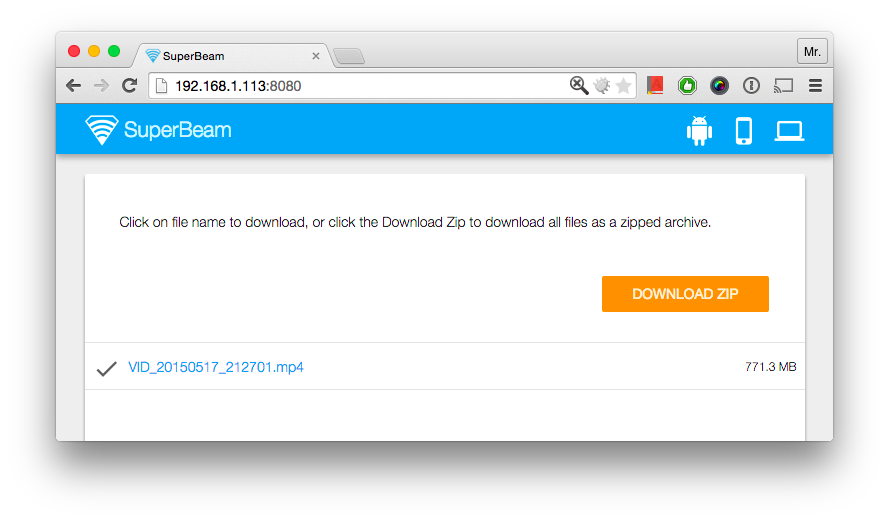
\includegraphics[width=0.9\textwidth]{images/alternatives/superbeam_web.png}
	\caption{SuperBeam Web-Frontend Ansicht}
\end{figure}

Bei den Tests wurden folgende Übertragungsgeschwindigkeiten gemessen (Filetransfer von $\approx770$\,MB):
\begin{table}[H]
	% style
	\small\sffamily\renewcommand{\arraystretch}{1.4}
	% caption
	\captionabove{\gls{wlanLabel} vs. Wi-Fi Direct}
	\begin{tabular}{lp{0.35\linewidth}p{0.30\linewidth}}
		\toprule
		Technologie & Bit & Byte\\
		\midrule
		\gls{wlanLabel} & 0.8 - 6.4 Mbit/s & 0.1 - 0.8\,MB/s\\
		Wi-Fi Direct & 46\,Mbit/s & 5.75\,MB/s\\
		\bottomrule
	\end{tabular}
\end{table}

Besonders auffallend sind die bleibenden Schwankungen bei der \gls{wlanLabel}-Übertragung.
Obwohl das \gls{wlanLabel}-Netzwerk nebst dem Datentransfer kaum belastet wurde, variiert die Geschwindigkeit dauernd (bis um das Achtfache des Minimums).
Selbstverständlich spielt die Distanz und die Abschottung zwischen \gls{apLabel} und Client eine erhebliche Rolle.
Die Distanz wurde jedoch nach dem ersten Test minimiert, indem beide Geräte direkt neben den \gls{apLabel} gelegt wurden.

Beim Wi-Fi Direct hat sich die Geschwindigkeit bei 46\,Mbit/s sehr rasch stabilisiert, was gegenüber der Verbindung mit dem \gls{apLabel} (mit durchschnittlich 3.6\,Mbit/s) eine über zwölffache schnellere Geschwindigkeit ermöglicht.
Dies reduziert die Wartezeit mit Wi-Fi Direct auf beinahe 8\,\%.

\subsection{NFC}
\gls{nfcLabel} ist seit 2002 spezifiziert und wurde 2006 erstmalig in einem Smartphone eingebaut.
Die Technologie erlaubt innerhalb von 10\,cm eine Datenübertragung von max. 424\,kbit/s.
Je nach Anwendungsfall kann die Reichweite auf einen Meter erweitert werden, wozu allerdings eine 1.5\,m hohe Antenne benötigt wird (dies kann z.B. in einem Warenhaus vorkommen).\footcite{Near_Field_Communication_Wikipedia_2015-05-22}

Die \gls{nfcLabel}-Technologie kann vor allem für bargeldloses Zahlen verwendet werden.
Aufgrund der tiefen Übertragungsrate eignet sich \gls{nfcLabel} nicht für den Austausch von gewöhnlichen Dateien (Bilder, Dokumente, etc.).
Zudem darf während der Übertragungen die maximale Reichweite nicht überschritten werden.
Diese Einschränkung kann für den Nutzer als unbequem empfunden werden.
Für die Übertragung kleiner Datenmengen (vor allem textbasierte Daten) wie Kontakte, Links oder Einstellungen, kann \gls{nfcLabel} genutzt werden. Allerdings ist eine Kommunikation zwischen verschiedenen Systemen oft nicht möglich, weil die Programme keine einheitlichen Schnittstellen anbieten.

\subsubsection{Vorteile}
Durch die stark beschränkte Reichweite, wird unerlaubter Zugriff praktisch verunmöglicht.
Die Nutzung ist sehr einfach gehalten: Es reicht der Kontakt der Geräte um Daten auszutauschen ("`\textit{beamen}"').
Die Technologie bietet sich für sicherheitsrelevante Übertragungen von kleinen Datenmengen an.
Einzelne \gls{rfidLabel}'s, die eine Identifizierung ermöglichen, können sehr günstig erworben werden.

\subsubsection{Nachteile}
\gls{nfcLabel} wurde als eigene Technologie neben dem existierenden Bluetooth und \gls{wlanLabel} entwickelt.
Dabei wurde bewusst ein eigener Anwendungsbereich anvisiert.
Die tiefe Datenübertragungsrate und die kurze Reichweite ist also eine gewollte Funktion, resp. ein akzeptierter Kompromiss und kein Nachteil.
Hingegen handelt es sich bei \gls{nfcLabel} um eine zertifizierte Technologie.
Gerade im Zusammenhang mit der raren Verbreitung, stellt diese Zertifizierung eine grosse Hürde für das Angebot von dieser Technologie dar.

% http://www.mobilepaymentstoday.com/blogs/ble-vs-nfc-the-future-of-mobile-consumer-engagement-now-infographic/


% \subsection{Bluetooth}

